\section{Model checking in \emph{Reprotool}.}

\subsection{Introduction to model checking in \emph{Reprotool}.}

\emph{Reprotool} project can contain many use-cases. Use-cases consist of use-case steps. You can assign annotaions to individual
use-case steps. These annotations are basicly boolean variables. When the \emph{Reprotool} performs model checking, it firstly
initializes all annotaion variables to boolean value false. It then starts executing use-cases. Executing a use-case means executing
its use-case steps. If a step with an annotation is being executed, the value of the corresponding  annotation variable is changed to true.
The annotaions in a \emph{Reprotool} project must adhere to the rules that are defined in the project as a set of temporal logic
formulas. When you run the model checking in \emph{Reprotool}, you are actually checking the validity of these temporal logic formulas.
By assigning new annotaions to use-case steps in the project, you are actually extending the set of logic formulas that will be verified
during the model checking process.

\subsection{Predefined \emph{Reprotool} annotaions an their semantics.}
In every \emph{Reprotool} project, there is already a set of predefined annotations that you can use. You can, however, define new
annotations and define their behaviour. The predefined annotations already have some predefined default behaviour.

\subsubsection {The \emph{open} and \emph{close} annotaions are bound by these rules:}

\begin{enumerate}
  \item After 'open' there should always be 'close'.
  \item No multi-open without close.
  \item No multi-close without open.
  \item First 'open' then 'close'.
\end{enumerate}

\subsubsection{The \emph{create} and \emph{use} annotaions are bound by these rules:}

\begin{enumerate}
  \item After 'create' there must be some branch containing 'use'.
  \item Only one 'create'.
  \item First 'create' then 'use'.
\end{enumerate}

\subsubsection{The special \emph{trace} and \emph{on} annotations}
These two annotations are special, you can not override their meaning. By using these annotations, you can conditionally prune the
execution tree of the model checker during the verification process. You will better understand their meaning when we demonstrate
their usage later in this chapter.

\subsection{Generating the NuSMV model}
To generate the \emph{NuSMV} model specification of the \emph{cityMap.swproj} project, right-click the file in the project explorer
and run the command \emph{Convert SW project to SMV}. Notice in the project explorer, that a new file \emph{cityMap.swproj.nusmv} has
been generated in the \emph{Citymap example} project directory. This file contains the model specification for the \emph{NuSMV} model checker.

Open the \emph{cityMap.swproj.nusmv} file. The file will be opened by our \mbox{\emph{NuSMVLang}} editor. Using this editor, it is possible to manualy edit the generated model.
There is a \emph{NuSMV Manual} in the documentation directory of the \emph{Reprotool} svn tree. Direct editing of this
file should however not be necessary.

\begin{figure}[ht]
  \centering
  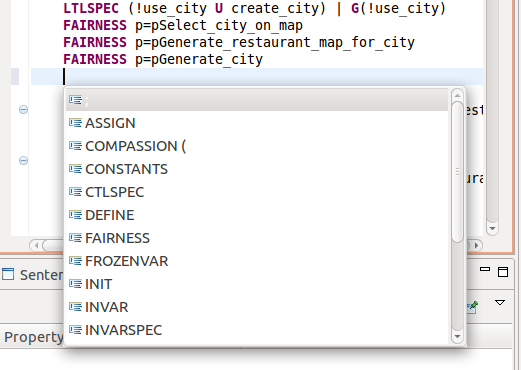
\includegraphics[height=180pt]{images/reprotoolNuSMVContentAssist}
  \caption{Content Assist in \emph{Reprotool} NuSMV editor}
  \label{fig:reprotoolNuSMVContentAssist}
\end{figure}

\hyphenation{Ve-ri-fi-ca-tion}

\subsection{Model checking}
To run the \emph{NuSMV} verification for the generated model \emph{cityMap.swproj.nusmv}, right-click this file in the project explorer
and run the command \emph{Run NuSMV Verification} from the context menu. The \emph{NuSMV} model checker now finds a violation of one of
the temporal logic formulas specified for this project and prints into the console the counter-example trace. This trace consists of
a series of state transitions as defined in the \emph{NuSMV} model file \emph{cityMap.swproj.nusmv} that leads to the violation.
A human-readable form of this trace is also generated. Notice the file \emph{cityMap.swproj.cexmp} that has been generated in the project
directory.

\subsection{Reading the counter-example trace}
Open the generated counter-example trace in the file \emph{cityMap.swproj.cexmp}. You should see a screen similar to this:

\begin{figure}[ht]
  \centering
  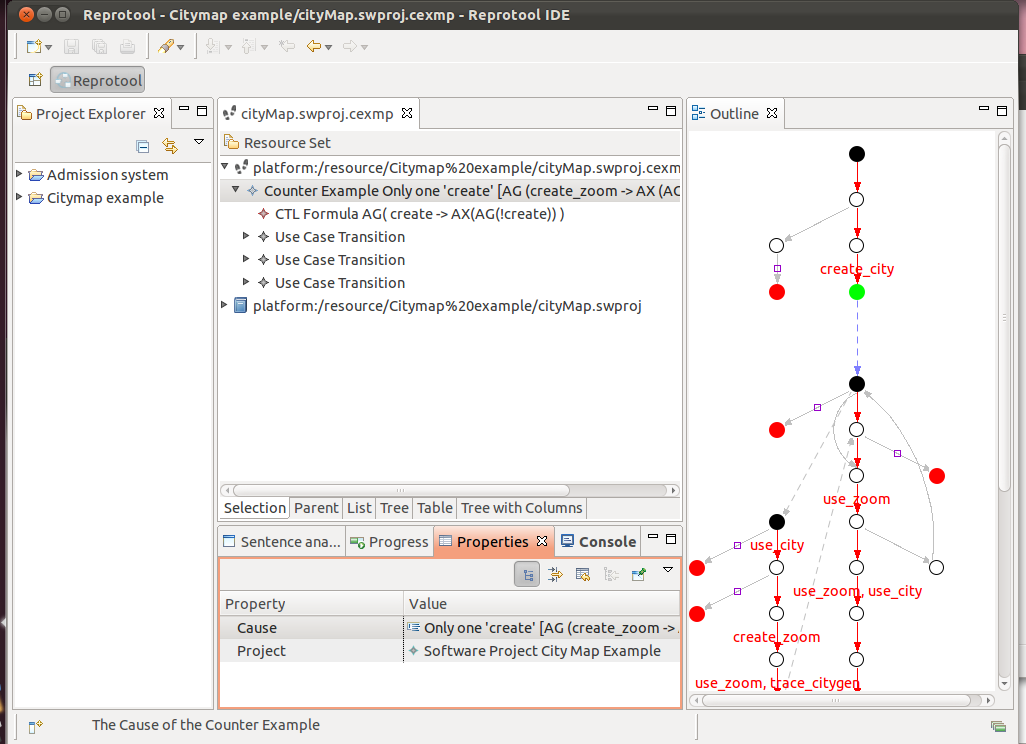
\includegraphics[height=280pt]{images/reprotoolTraceCityMap}
  \caption{Counter-example trace of the cityMap project}
  \label{fig:reprotoolTraceCityMap}
\end{figure}

Make sure that the outline and the properties views are visible. You can see the visual representation of the execution path in the
outline view. What we are going to find out by inspecting this trace is the temporal property that has been violated.
Click on the root \emph{Counter Example} tree node in the editor view that shows the counter-example trace. In the properties view,
you can see the \emph{Project} property that tells us for which project the counter-example has been generated. There is also the
\emph{Cuase} property that reads:
\begin{verbatim}
Only one 'create' [AG (create_zoom -> AX (AG !create_zoom)) ]
\end{verbatim}
This line contains the temporal logic formula description and then the actual formula in the square brackets. From the formula
description, we see that the problem is that some object has been created more than once. And from the actual formula, we can
see that the \emph{zoom} object is the one that has been created more than once. Now look carefully into the outline view and
follow the red line that shows us the execution path. You will see, that indeed the \emph{create\_zoom} annotaion appears two times
in the trace. And this causes the violation of the shown temporal logic formula.

From this counter-example trace, you can see the order in which the individual use-cases have been executed. This corresponds to the
order of use-case transitions in the counter-example trace. Every use-case transition node corresponds to a single execution path inside
the specified use-case. By selecting the \emph{Use Case Transition} node in the editor view and inspecting the properties sheet, you can
view the use-case that this transition represents. Inside this \emph{Use Case Transition} tree node, you can see the \emph{Step} nodes
that represent the individual use-case steps performed during execution of the use-case. These \emph{Step} nodes can be either leaf
nodes - if they represent a simple use-case step. \emph{Step} node can also have a child \emph{Use Case Transition} node if the step
includes another use-case.

\subsection{Fixing the annotaions in the \emph{Citymap example} project.}

Open the counter-example trace \emph{cityMap.swproj.cexmp} of the \emph{Citymap example} project. From the previous section, we already
know that the problem is caused by the \emph{create\_zoom} annotaion. Locate the use-case that contains the step with this annotation.
You should now be able to find out, that this use-case step is part of the \emph{Generate city} use-case. Choose one step from this
use-case and double-click it. You can double-click it either in the outline view, or in the editor view.

The use-case editor with the \emph{Generate city} use-case will fire up. The problem is with the step 3 that contains the \emph{create\_zoom}
annotation. This use-case is executed once as a stand-alone use-case, and once as the part of the \emph{Generate restaurant map for
the city} use-case that includes the \emph{Generate city} use-case. That is why the \emph{create\_zoom} annotation appears two times.

This is how we are going to fix it: We will add a branch after the use-case step 2 that will lead to the use-case abortion. And we will
specify that this branch will be taken if and only if the \emph{Generate city} use-case has been already executed. This way,
the \emph{create\_zoom} annotaion will appear only once. Because during the second execution of the use-case, before the
\emph{create\_zoom} annotaion can appear, our branch will be taken and the use-case will abort.

Adding the branching is easy. We will add an extension scenario to the step 2. Select this step in the use-case editor and press
\texttt{Ctrl + 1}. This will create a new extension scenario for the selected step. The newly created step has label \emph{2a1}.
Type the sentence \emph{Abort use-case} as the text for this step. Now click the lightning icon in the toolbar area that causes
the linguistic analysis of the selected step. You will learn more about linguistic analysis in \emph{Reprotool} in a later chapter
devoted to this topic. Check in the sentence-analysis view, that the step has defined its action type as \emph{Abort use-case}.
You can notice it also in the outline view. Anyway, you should now be in a situation similar to this:

\begin{figure}[ht]
  \centering
  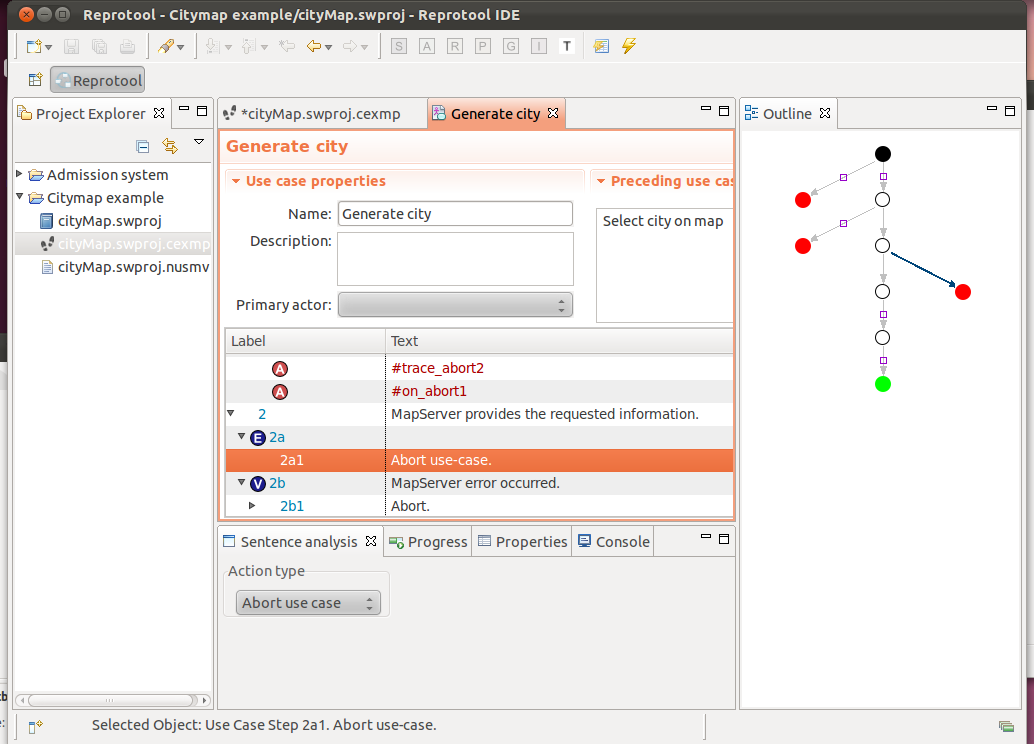
\includegraphics[height=280pt]{images/reprotoolTraceCityMapFix1}
  \caption{Added extension scenario with abort action to the step 2.}
  \label{fig:reprotoolTraceCityMapFix1}
\end{figure}

So we have already created the branching that we need. Now we need to somehow specify that this branching must be taken if and
only if the \emph{Generate city} use-case has been previously executed. For this, we will use the special annotaions.

\subsubsection{Special annotaions \emph{trace} and \emph{on}.}
\begin{definition}[Semantics of the trace-on annotation pair]
	Let $S$ be a a use-case step.
	Let $on\_x$ be an annotation attached to $S$ (\emph{x} is and arbitrary annotation id).
	Let $T=\{t: S \in t\}$ be a set of all traces going through the step $S$.
	A trace $t \in T$ will be considered for verification only if it contains a step $R'$ annotated with $trace\_x$ before the step $S$.
\end{definition}

This means that: If we have in our project a use-case step for which we want to ask \emph{Have we already visited this step?} then
we attach a \emph{trace} annotaion to this step. Later in some branching we can specify which branch to take based on the answer
to that question. We can attach the \emph{on} annotaion to the first step of the branch. This branch will be taken if and only if
the \emph{trace} annotaion has been previously encountered.

The \emph{trace} and \emph{on} annotaions are identified by unique ids. This enables us to use more \emph{trace / on} annotaion
pairs in the project.

Now we go back to our \emph{Citymap example} project. Notice that the step 4 of the \emph{Generate city} use-case is annotated
with the \emph{trace\_citygen} annotaion. So all we need to do is to attach the \emph{on\_citygen} annotaion to the branching
step with label \emph{2a1} that we have just created. To do this, firstly make sure that the properties view is displayed and
then select the step with the label \emph{2a1} in the use-case editor. Now, press \texttt{Ctrl + 4} on your keyboard. This will
add an annotaion to this step. Now, select the annotaion in the editor and type the \emph{citygen} as annotation id in the
properties view. Now, select \emph{Special annotaion on} as the annotaion type in the properties view. You should be in a
situation similar to this:

\begin{figure}[ht]
  \centering
  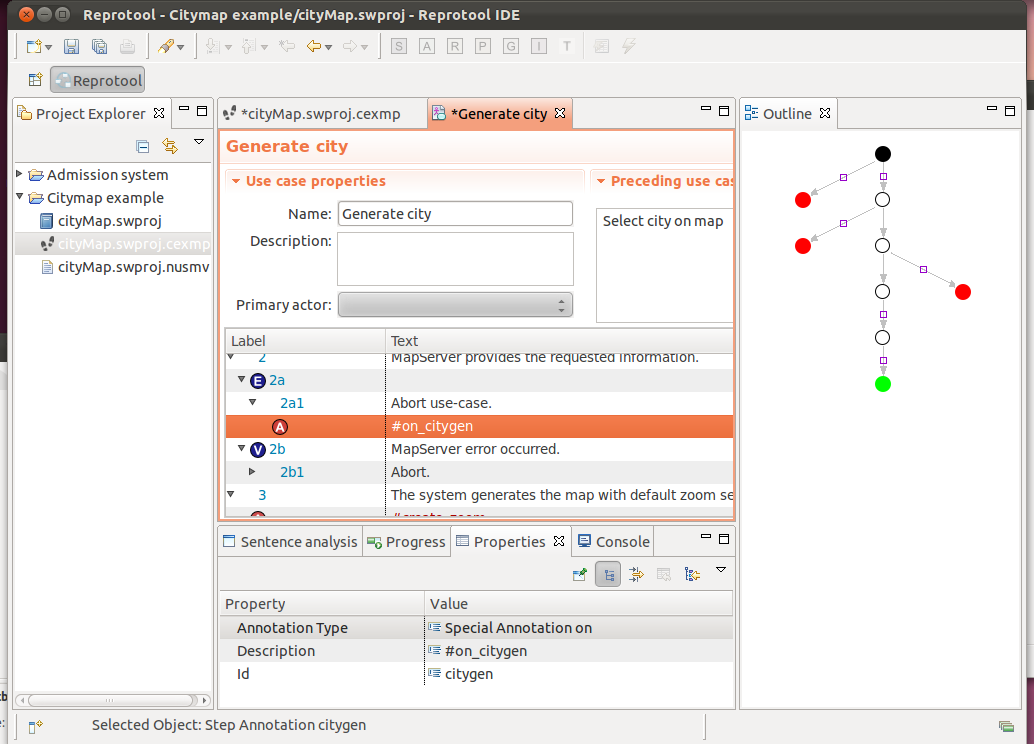
\includegraphics[height=280pt]{images/reprotoolTraceCityMapFix2}
  \caption{Added special \emph{on} annotation to the step \emph{2a1}.}
  \label{fig:reprotoolTraceCityMapFix2}
\end{figure}

Now we are finished. Run the verification again, and you should see in the console view that none of the temporal logic properties
has been violated.